\chapter{Recorrido de grafos}

Este capítulo trata dos algoritmos
fundamentales de grafos:
la búsqueda en profundidad y la búsqueda en anchura.
A ambos algoritmos se les da un nodo
inicial en el grafo,
y visitan todos los nodos que se pueden alcanzar
desde el nodo inicial.
La diferencia entre los algoritmos es el orden
en el que visitan los nodos.

\section{Búsqueda en profundidad}

\index{búsqueda en profundidad}

La \key{búsqueda en profundidad} (DFS)
es una técnica sencilla de recorrido de grafos.
El algoritmo comienza en un nodo inicial,
y avanza hacia todos los demás nodos que son
alcanzables desde el nodo inicial usando
las aristas del grafo.

La búsqueda en profundidad siempre sigue un único
camino en el grafo mientras encuentra
nodos nuevos.
Después de esto, regresa a los nodos
anteriores y comienza a explorar otras partes del grafo.
El algoritmo lleva un registro de los nodos visitados,
de manera que procesa cada nodo solo una vez.

\subsubsection*{Ejemplo}

Consideremos cómo la búsqueda en profundidad procesa
el siguiente grafo:
\begin{center}
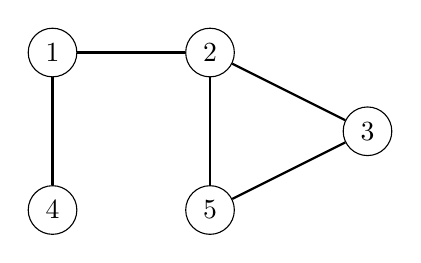
\begin{tikzpicture}
\node[draw, circle] (1) at (1,5) {$1$};
\node[draw, circle] (2) at (3,5) {$2$};
\node[draw, circle] (3) at (5,4) {$3$};
\node[draw, circle] (4) at (1,3) {$4$};
\node[draw, circle] (5) at (3,3) {$5$};

\path[draw,thick,-] (1) -- (2);
\path[draw,thick,-] (2) -- (3);
\path[draw,thick,-] (1) -- (4);
\path[draw,thick,-] (3) -- (5);
\path[draw,thick,-] (2) -- (5);
\end{tikzpicture}
\end{center}
Podemos comenzar la búsqueda en cualquier nodo del grafo;
ahora comenzaremos la búsqueda en el nodo 1.

La búsqueda avanza primero al nodo 2:
\begin{center}
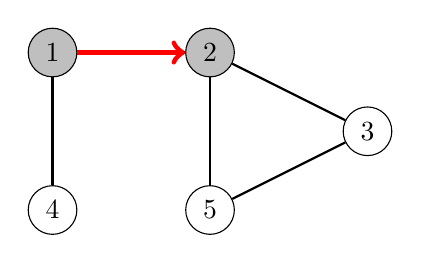
\begin{tikzpicture}
\node[draw, circle,fill=lightgray] (1) at (1,5) {$1$};
\node[draw, circle,fill=lightgray] (2) at (3,5) {$2$};
\node[draw, circle] (3) at (5,4) {$3$};
\node[draw, circle] (4) at (1,3) {$4$};
\node[draw, circle] (5) at (3,3) {$5$};

\path[draw,thick,-] (1) -- (2);
\path[draw,thick,-] (2) -- (3);
\path[draw,thick,-] (1) -- (4);
\path[draw,thick,-] (3) -- (5);
\path[draw,thick,-] (2) -- (5);

\path[draw=red,thick,->,line width=2pt] (1) -- (2);
\end{tikzpicture}
\end{center}
Después de esto, se visitarán los nodos 3 y 5:
\begin{center}
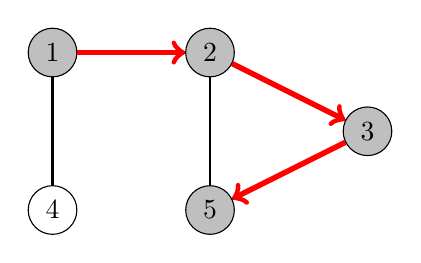
\begin{tikzpicture}
\node[draw, circle,fill=lightgray] (1) at (1,5) {$1$};
\node[draw, circle,fill=lightgray] (2) at (3,5) {$2$};
\node[draw, circle,fill=lightgray] (3) at (5,4) {$3$};
\node[draw, circle] (4) at (1,3) {$4$};
\node[draw, circle,fill=lightgray] (5) at (3,3) {$5$};

\path[draw,thick,-] (1) -- (2);
\path[draw,thick,-] (2) -- (3);
\path[draw,thick,-] (1) -- (4);
\path[draw,thick,-] (3) -- (5);
\path[draw,thick,-] (2) -- (5);

\path[draw=red,thick,->,line width=2pt] (1) -- (2);
\path[draw=red,thick,->,line width=2pt] (2) -- (3);
\path[draw=red,thick,->,line width=2pt] (3) -- (5);
\end{tikzpicture}
\end{center}
Los vecinos del nodo 5 son 2 y 3,
pero la búsqueda ya ha visitado ambos,
así que es momento de regresar a los nodos anteriores.
También se han visitado los vecinos de los nodos 3 y 2,
así que a continuación nos movemos
del nodo 1 al nodo 4:
\begin{center}
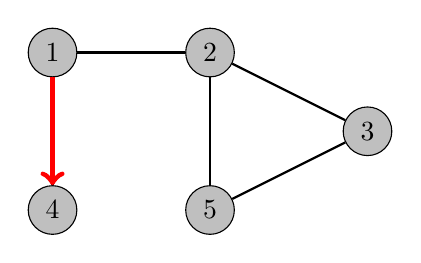
\begin{tikzpicture}
\node[draw, circle,fill=lightgray] (1) at (1,5) {$1$};
\node[draw, circle,fill=lightgray] (2) at (3,5) {$2$};
\node[draw, circle,fill=lightgray] (3) at (5,4) {$3$};
\node[draw, circle,fill=lightgray] (4) at (1,3) {$4$};
\node[draw, circle,fill=lightgray] (5) at (3,3) {$5$};

\path[draw,thick,-] (1) -- (2);
\path[draw,thick,-] (2) -- (3);
\path[draw,thick,-] (1) -- (4);
\path[draw,thick,-] (3) -- (5);
\path[draw,thick,-] (2) -- (5);

\path[draw=red,thick,->,line width=2pt] (1) -- (4);
\end{tikzpicture}
\end{center}
Después de esto, la búsqueda termina porque ha visitado
todos los nodos.

La complejidad temporal de la búsqueda en profundidad es $O(n+m)$
donde $n$ es el número de nodos y $m$ es el
número de aristas,
porque el algoritmo procesa cada nodo y arista una vez.

\subsubsection*{Implementación}

La búsqueda en profundidad se puede
implementar cómodamente usando recursión.
La siguiente función \texttt{dfs} comienza
una búsqueda en profundidad en un nodo dado.
La función supone que el grafo está
almacenado como listas de adyacencia en un arreglo
\begin{lstlisting}
vector<int> adj[N];
\end{lstlisting}
y también mantiene un arreglo
\begin{lstlisting}
bool visited[N];
\end{lstlisting}
que lleva un registro de los nodos visitados.
Inicialmente, cada valor del arreglo es \texttt{false},
y cuando la búsqueda llega al nodo $s$,
el valor de \texttt{visited}[$s$] pasa a ser \texttt{true}.
La función se puede implementar como sigue:
\begin{lstlisting}
void dfs(int s) {
    if (visited[s]) return;
    visited[s] = true;
    // process node s
    for (auto u: adj[s]) {
        dfs(u);
    }
}
\end{lstlisting}

\section{Búsqueda en anchura}

\index{búsqueda en anchura}

La \key{búsqueda en anchura} (BFS) visita los nodos
en orden creciente de su distancia
desde el nodo inicial.
Así, podemos calcular la distancia
desde el nodo inicial a todos los demás
nodos usando la búsqueda en anchura.
Sin embargo, la búsqueda en anchura es más difícil
de implementar que la búsqueda en profundidad.

La búsqueda en anchura recorre los nodos
un nivel tras otro.
Primero la búsqueda explora los nodos cuya
distancia desde el nodo inicial es 1,
luego los nodos cuya distancia es 2, y así sucesivamente.
Este proceso continúa hasta que todos los nodos
han sido visitados.

\subsubsection*{Ejemplo}

Consideremos cómo la búsqueda en anchura procesa
el siguiente grafo:

\begin{center}
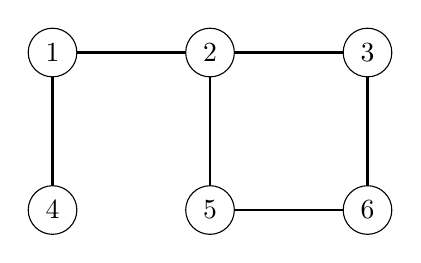
\begin{tikzpicture}
\node[draw, circle] (1) at (1,5) {$1$};
\node[draw, circle] (2) at (3,5) {$2$};
\node[draw, circle] (3) at (5,5) {$3$};
\node[draw, circle] (4) at (1,3) {$4$};
\node[draw, circle] (5) at (3,3) {$5$};
\node[draw, circle] (6) at (5,3) {$6$};

\path[draw,thick,-] (1) -- (2);
\path[draw,thick,-] (2) -- (3);
\path[draw,thick,-] (1) -- (4);
\path[draw,thick,-] (3) -- (6);
\path[draw,thick,-] (2) -- (5);
\path[draw,thick,-] (5) -- (6);
\end{tikzpicture}
\end{center}
Supongamos que la búsqueda comienza en el nodo 1.
Primero, procesamos todos los nodos que se pueden alcanzar
desde el nodo 1 usando una sola arista:
\begin{center}
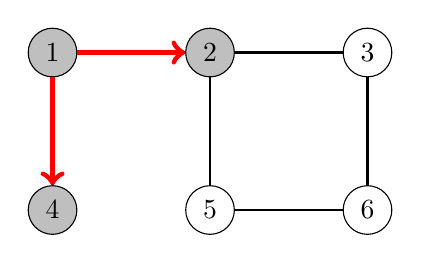
\begin{tikzpicture}
\node[draw, circle,fill=lightgray] (1) at (1,5) {$1$};
\node[draw, circle,fill=lightgray] (2) at (3,5) {$2$};
\node[draw, circle] (3) at (5,5) {$3$};
\node[draw, circle,fill=lightgray] (4) at (1,3) {$4$};
\node[draw, circle] (5) at (3,3) {$5$};
\node[draw, circle] (6) at (5,3) {$6$};

\path[draw,thick,-] (1) -- (2);
\path[draw,thick,-] (2) -- (3);
\path[draw,thick,-] (1) -- (4);
\path[draw,thick,-] (3) -- (6);
\path[draw,thick,-] (2) -- (5);
\path[draw,thick,-] (5) -- (6);

\path[draw,thick,-] (1) -- (2);
\path[draw,thick,-] (2) -- (3);
\path[draw,thick,-] (1) -- (4);
\path[draw,thick,-] (2) -- (5);

\path[draw=red,thick,->,line width=2pt] (1) -- (2);
\path[draw=red,thick,->,line width=2pt] (1) -- (4);
\end{tikzpicture}
\end{center}
Después de esto, avanzamos a los nodos 3 y 5:
\begin{center}
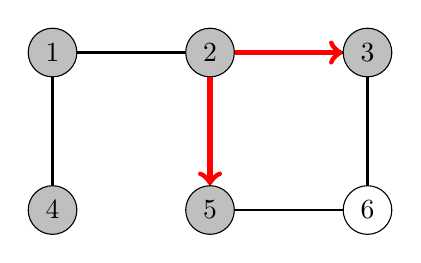
\begin{tikzpicture}
\node[draw, circle,fill=lightgray] (1) at (1,5) {$1$};
\node[draw, circle,fill=lightgray] (2) at (3,5) {$2$};
\node[draw, circle,fill=lightgray] (3) at (5,5) {$3$};
\node[draw, circle,fill=lightgray] (4) at (1,3) {$4$};
\node[draw, circle,fill=lightgray] (5) at (3,3) {$5$};
\node[draw, circle] (6) at (5,3) {$6$};

\path[draw,thick,-] (1) -- (2);
\path[draw,thick,-] (2) -- (3);
\path[draw,thick,-] (1) -- (4);
\path[draw,thick,-] (3) -- (6);
\path[draw,thick,-] (2) -- (5);
\path[draw,thick,-] (5) -- (6);

\path[draw,thick,-] (1) -- (2);
\path[draw,thick,-] (2) -- (3);
\path[draw,thick,-] (1) -- (4);
\path[draw,thick,-] (2) -- (5);

\path[draw=red,thick,->,line width=2pt] (2) -- (3);
\path[draw=red,thick,->,line width=2pt] (2) -- (5);
\end{tikzpicture}
\end{center}
Finalmente, visitamos el nodo 6:
\begin{center}
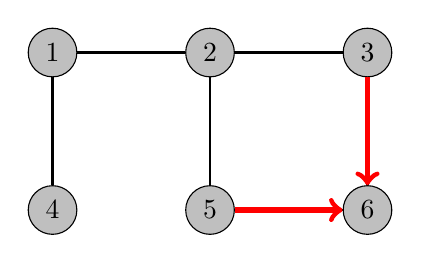
\begin{tikzpicture}
\node[draw, circle,fill=lightgray] (1) at (1,5) {$1$};
\node[draw, circle,fill=lightgray] (2) at (3,5) {$2$};
\node[draw, circle,fill=lightgray] (3) at (5,5) {$3$};
\node[draw, circle,fill=lightgray] (4) at (1,3) {$4$};
\node[draw, circle,fill=lightgray] (5) at (3,3) {$5$};
\node[draw, circle,fill=lightgray] (6) at (5,3) {$6$};

\path[draw,thick,-] (1) -- (2);
\path[draw,thick,-] (2) -- (3);
\path[draw,thick,-] (1) -- (4);
\path[draw,thick,-] (3) -- (6);
\path[draw,thick,-] (2) -- (5);
\path[draw,thick,-] (5) -- (6);

\path[draw,thick,-] (1) -- (2);
\path[draw,thick,-] (2) -- (3);
\path[draw,thick,-] (1) -- (4);
\path[draw,thick,-] (2) -- (5);

\path[draw=red,thick,->,line width=2pt] (3) -- (6);
\path[draw=red,thick,->,line width=2pt] (5) -- (6);
\end{tikzpicture}
\end{center}
Ahora hemos calculado las distancias
desde el nodo inicial a todos los nodos del grafo.
Las distancias son las siguientes:

\begin{tabular}{ll}
\\
nodo & distancia \\
\hline
1 & 0 \\
2 & 1 \\
3 & 2 \\
4 & 1 \\
5 & 2 \\
6 & 3 \\
\\
\end{tabular}

Al igual que en la búsqueda en profundidad,
la complejidad temporal de la búsqueda en anchura
es $O(n+m)$, donde $n$ es el número de nodos
y $m$ es el número de aristas.

\subsubsection*{Implementación}

La búsqueda en anchura es más difícil
de implementar que la búsqueda en profundidad,
porque el algoritmo visita nodos
en diferentes partes del grafo.
Una implementación típica se basa en
una cola que contiene nodos.
En cada paso, se procesará el siguiente nodo
de la cola.

El siguiente código supone que el grafo está almacenado
como listas de adyacencia y mantiene las siguientes
estructuras de datos:
\begin{lstlisting}
queue<int> q;
bool visited[N];
int distance[N];
\end{lstlisting}

La cola \texttt{q}
contiene los nodos a procesar
en orden creciente de su distancia.
Los nodos nuevos siempre se añaden al final
de la cola, y el nodo al principio
de la cola es el siguiente nodo a procesar.
El arreglo \texttt{visited} indica
qué nodos ha visitado ya la búsqueda,
y el arreglo \texttt{distance} contendrá las
distancias desde el nodo inicial a todos los nodos del grafo.

La búsqueda se puede implementar como sigue,
comenzando en el nodo $x$:
\begin{lstlisting}
visited[x] = true;
distance[x] = 0;
q.push(x);
while (!q.empty()) {
    int s = q.front(); q.pop();
    // process node s
    for (auto u : adj[s]) {
        if (visited[u]) continue;
        visited[u] = true;
        distance[u] = distance[s]+1;
        q.push(u);
    }
}
\end{lstlisting}

\section{Aplicaciones}

Usando los algoritmos de recorrido de grafos,
podemos comprobar muchas propiedades de los grafos.
Usualmente, tanto la búsqueda en profundidad como
la búsqueda en anchura se pueden usar,
pero en la práctica, la búsqueda en profundidad
es una mejor elección, porque es
más fácil de implementar.
En las siguientes aplicaciones
supondremos que el grafo es no dirigido.

\subsubsection{Comprobación de conectividad}

\index{grafo conexo}

Un grafo es conexo si hay un camino
entre cualesquiera dos nodos del grafo.
Así, podemos comprobar si un grafo es conexo
comenzando en un nodo arbitrario y
averiguando si podemos alcanzar todos los demás nodos.

Por ejemplo, en el grafo
\begin{center}
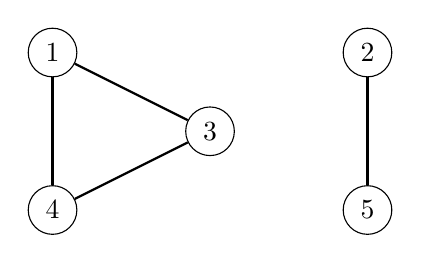
\begin{tikzpicture}
\node[draw, circle] (2) at (7,5) {$2$};
\node[draw, circle] (1) at (3,5) {$1$};
\node[draw, circle] (3) at (5,4) {$3$};
\node[draw, circle] (5) at (7,3) {$5$};
\node[draw, circle] (4) at (3,3) {$4$};

\path[draw,thick,-] (1) -- (3);
\path[draw,thick,-] (1) -- (4);
\path[draw,thick,-] (3) -- (4);
\path[draw,thick,-] (2) -- (5);
\end{tikzpicture}
\end{center}
una búsqueda en profundidad desde el nodo $1$ visita
los siguientes nodos:
\begin{center}
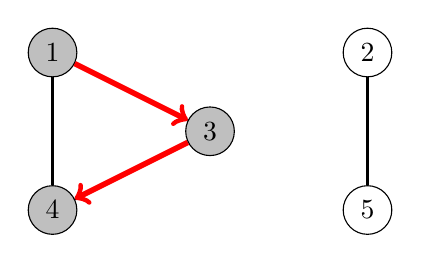
\begin{tikzpicture}
\node[draw, circle] (2) at (7,5) {$2$};
\node[draw, circle,fill=lightgray] (1) at (3,5) {$1$};
\node[draw, circle,fill=lightgray] (3) at (5,4) {$3$};
\node[draw, circle] (5) at (7,3) {$5$};
\node[draw, circle,fill=lightgray] (4) at (3,3) {$4$};

\path[draw,thick,-] (1) -- (3);
\path[draw,thick,-] (1) -- (4);
\path[draw,thick,-] (3) -- (4);
\path[draw,thick,-] (2) -- (5);

\path[draw=red,thick,->,line width=2pt] (1) -- (3);
\path[draw=red,thick,->,line width=2pt] (3) -- (4);

\end{tikzpicture}
\end{center}

Como la búsqueda no visitó todos los nodos,
podemos concluir que el grafo no es conexo.
De manera similar, también podemos encontrar todos los componentes conexos
de un grafo iterando por los nodos y siempre
comenzando una nueva búsqueda en profundidad si el nodo actual
no pertenece todavía a ningún componente.

\subsubsection{Búsqueda de ciclos}

\index{ciclo}

Un grafo contiene un ciclo si durante un recorrido del grafo,
encontramos un nodo cuyo vecino (distinto del
nodo anterior en el camino actual) ya ha sido
visitado.
Por ejemplo, el grafo
\begin{center}
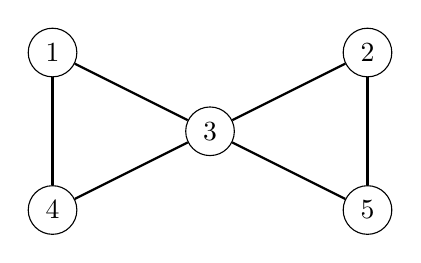
\begin{tikzpicture}
\node[draw, circle] (2) at (7,5) {$2$};
\node[draw, circle] (1) at (3,5) {$1$};
\node[draw, circle] (3) at (5,4) {$3$};
\node[draw, circle] (5) at (7,3) {$5$};
\node[draw, circle] (4) at (3,3) {$4$};

\path[draw,thick,-] (1) -- (3);
\path[draw,thick,-] (1) -- (4);
\path[draw,thick,-] (3) -- (4);
\path[draw,thick,-] (2) -- (5);
\path[draw,thick,-] (2) -- (3);
\path[draw,thick,-] (3) -- (5);
\end{tikzpicture}
\end{center}
contiene dos ciclos y podemos encontrar uno
de ellos como sigue:
\begin{center}
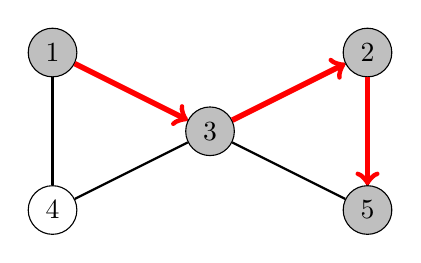
\begin{tikzpicture}
\node[draw, circle,fill=lightgray] (2) at (7,5) {$2$};
\node[draw, circle,fill=lightgray] (1) at (3,5) {$1$};
\node[draw, circle,fill=lightgray] (3) at (5,4) {$3$};
\node[draw, circle,fill=lightgray] (5) at (7,3) {$5$};
\node[draw, circle] (4) at (3,3) {$4$};

\path[draw,thick,-] (1) -- (3);
\path[draw,thick,-] (1) -- (4);
\path[draw,thick,-] (3) -- (4);
\path[draw,thick,-] (2) -- (5);
\path[draw,thick,-] (2) -- (3);
\path[draw,thick,-] (3) -- (5);

\path[draw=red,thick,->,line width=2pt] (1) -- (3);
\path[draw=red,thick,->,line width=2pt] (3) -- (2);
\path[draw=red,thick,->,line width=2pt] (2) -- (5);

\end{tikzpicture}
\end{center}
Después de movernos del nodo 2 al nodo 5 notamos que
el vecino 3 del nodo 5 ya ha sido visitado.
Así, el grafo contiene un ciclo que pasa por el nodo 3,
por ejemplo, $3 \rightarrow 2 \rightarrow 5 \rightarrow 3$.

Otra forma de averiguar si un grafo contiene un ciclo
es simplemente calcular el número de nodos y aristas
en cada componente.
Si un componente contiene $c$ nodos y ningún ciclo,
debe contener exactamente $c-1$ aristas
(así que tiene que ser un árbol).
Si hay $c$ o más aristas, el componente
seguramente contiene un ciclo.

\subsubsection{Comprobación de bipartición}

\index{grafo bipartito}

Un grafo es bipartito si sus nodos se pueden colorear
usando dos colores de manera que no haya nodos
adyacentes con el mismo color.
Es sorprendentemente fácil comprobar si un grafo
es bipartito usando algoritmos de recorrido de grafos.

La idea es colorear el nodo inicial de azul,
todos sus vecinos de rojo, todos los vecinos de estos de azul, y así sucesivamente.
Si en algún punto de la búsqueda notamos que
dos nodos adyacentes tienen el mismo color,
esto significa que el grafo no es bipartito.
En caso contrario el grafo es bipartito y se ha encontrado
una coloración.

Por ejemplo, el grafo
\begin{center}
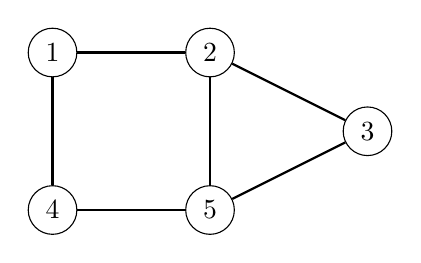
\begin{tikzpicture}
\node[draw, circle] (2) at (5,5) {$2$};
\node[draw, circle] (1) at (3,5) {$1$};
\node[draw, circle] (3) at (7,4) {$3$};
\node[draw, circle] (5) at (5,3) {$5$};
\node[draw, circle] (4) at (3,3) {$4$};

\path[draw,thick,-] (1) -- (2);
\path[draw,thick,-] (2) -- (5);
\path[draw,thick,-] (5) -- (4);
\path[draw,thick,-] (4) -- (1);
\path[draw,thick,-] (2) -- (3);
\path[draw,thick,-] (5) -- (3);
\end{tikzpicture}
\end{center}
no es bipartito, porque una búsqueda desde el nodo 1
procede como sigue:
\begin{center}
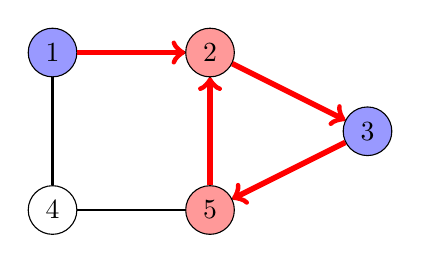
\begin{tikzpicture}
\node[draw, circle,fill=red!40] (2) at (5,5) {$2$};
\node[draw, circle,fill=blue!40] (1) at (3,5) {$1$};
\node[draw, circle,fill=blue!40] (3) at (7,4) {$3$};
\node[draw, circle,fill=red!40] (5) at (5,3) {$5$};
\node[draw, circle] (4) at (3,3) {$4$};

\path[draw,thick,-] (1) -- (2);
\path[draw,thick,-] (2) -- (5);
\path[draw,thick,-] (5) -- (4);
\path[draw,thick,-] (4) -- (1);
\path[draw,thick,-] (2) -- (3);
\path[draw,thick,-] (5) -- (3);

\path[draw=red,thick,->,line width=2pt] (1) -- (2);
\path[draw=red,thick,->,line width=2pt] (2) -- (3);
\path[draw=red,thick,->,line width=2pt] (3) -- (5);
\path[draw=red,thick,->,line width=2pt] (5) -- (2);
\end{tikzpicture}
\end{center}
Notamos que el color tanto del nodo 2 como del nodo 5
es rojo, mientras que son nodos adyacentes en el grafo.
Así, el grafo no es bipartito.

Este algoritmo siempre funciona, porque cuando
solo hay dos colores disponibles,
el color del nodo inicial en un componente
determina los colores de todos los demás nodos del componente.
No hay ninguna diferencia si el
nodo inicial es rojo o azul.

Nótese que en el caso general,
es difícil averiguar si los nodos
de un grafo se pueden colorear usando $k$ colores
de manera que no haya nodos adyacentes con el mismo color.
Incluso cuando $k=3$, no se conoce ningún algoritmo eficiente
sino que el problema es NP-difícil.
